%!TEX root = ../Report.tex
\subsection{System Architecture} % (fold)
\label{sub:system_architecture}
	\begin{figure}[h]
		\centering
		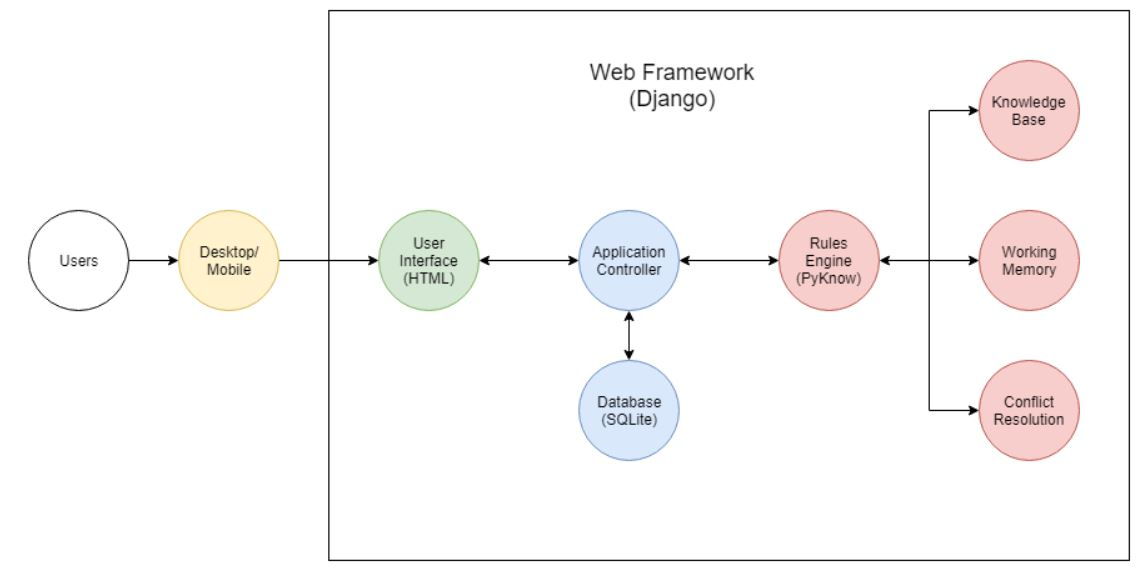
\includegraphics[width=\linewidth]{img/SystemArchitectureDiagram1a.jpg}
		\caption{System Architecture Diagram}
		\label{fig:system_architecture_diagram}
	\end{figure}
	Figure \ref{fig:system_architecture_diagram} shows the system architecture diagram of our recommender system. It illustrates how the different components interact with each other through the Django web framework. After the user keys in the inputs in the User Interface, it will be passed through the Django framework to the rules engine, PyKnow, which will perform the reasoning portion of the system, for example the calculation of cashback and rewards. The rules engine will then return the results to be matched against the database, with the final recommendation being passed back to the HTML page to be displayed.

% subsection system_architecture (end)

\subsection{Project Scope} % (fold)
\label{sub:project_scope}
While banks regularly have promotions for their credit cards to try and incentivise consumers to choose them and the additional rewards, our recommender system will only recommend credit cards based on their default rates/fees. This is so that the system can generally be applicable at all periods, regardless of seasonal promotional timeframes.

The banks chosen for this project are the main banks operating in Singapore, which covers what the majority of consumers in Singapore are using. This knowledge is also something which we extracted from our survey results.

The banks chosen are DBS, OCBC, UOB, HSBC, Maybank, Citibank and Standard Chartered.
% subsection project_scope (end)


\subsection{Assumptions} % (fold)
\label{sub:assumptions}

	\subsubsection{Eligibility of Users} % (fold)
	\label{ssub:eligibility_of_users}
	The major target audience would be the people spending most money in Singapore locally (including online). The user tracks his spending habits with cards (cashless). The user will pay fully before due date, i.e\ no late payment fee was considered.

	The user is able to successfully apply the card if he reaches the salary requirement (no bad credit history). Although the bank may approve the application even the user does not match the criteria provided by the bank, we still assume the bank would strictly follow the requirement bases on their official website.

	% subsubsection eligibility_of_users (end)

	\subsubsection{Knowledge Acquisition} % (fold)
	\label{ssub:knowledge_acquisition}
	Credit cards data are mainly from \href{https://www.moneysmart.sg/credit-cards}{MoneySmart}. It is assumed the data provided by this website is correct. The official website of bank might be used to check some detailed information.

	% subsubsection knowledge_acquisition (end)


% subsection assumptions (end)

\subsection{System Features} % (fold)
\label{sub:system_features}

	\subsubsection{Highly Personalized} % (fold)
	\label{ssub:highly_personalized}
	MRCard is highly personlized for each user, no matter the user is a consumer or a bank.

	People from general punlic have their own preferences and spending habits. MRCard would match the user's situation to provide the most recommended card. The user would also get the ideal card based on his spending habits without his preferences constraints. This would provide more useful information which the user may not realize before.

	As it is also a system can be applied by banks, the bank would get to understand how they should recommend the card based on the consumer's requirement. It would also give the bank a chance to see what their competing product is so they can develop a strategy to get consumers.

	% subsubsection highly_personalized (end)

	\subsubsection{Ease of Access} % (fold)
	\label{ssub:ease_of_access}

	MRCard is built on a web-based application. After the deployment on a server, the user can easily access it from a browser with Internet connection.

	Based on the bootstrap framework, MRCard is mobile friendly and can dynamically fit different screen sizes. The user can use it directly from their mobile phone. If the bank wants to provide MRCard as a service in their branches, only a tablet is needed for on-site employees and customers.

	% subsubsection ease_of_access (end)

% subsection system_features (end)

\subsection{Limitations} % (fold)
\label{sub:limitations}

As \href{https://www.moneysmart.sg/credit-cards}{MoneySmart} only covers most popular credit cards in Singapore, some credit cards may not be included for the recommendation.

To simplify the calculation, only long term major features of the cards were included. Some would be manually converted to cash value for comparison.

As there are some special credit cards for specific groups of people, these cards are excluded in the system. The system also excludes all special term for special employee benefits.

% subsection limitations (end)